\documentclass[a4paper]{article}

\usepackage[english]{babel}
\usepackage[utf8]{inputenc}
\usepackage{amsmath}
\usepackage{hyperref}
\usepackage{graphicx}
\usepackage[colorinlistoftodos]{todonotes}

\title{Q3. Numerical Integration: (Dr. Shanbhag )}

\author{Amirhessam Tahmassebi}

\date{\today}

\begin{document}
\maketitle



\section{Method}

For this problem, I used MCMC method. I have used Dr. Sachin's notes for MCMC class. Here is the link:
\href{https://sites.google.com/site/drsachinshanbhag/teaching/isc-5228}MCMC NOTES \newline
We have also the notes online at
\href{https://github.com/FSUSciComp/lecture-notes/tree/master/MCMC}Github.com/FSUSciComp. \newline
For this problem, we have a probability distribution function $\pi (X,Y)$. Using MCMC we will throw some sample points (like 10000) to find some points which work for our distribution function.
To find expectation value of $X$ we can find the mean value of $X$ coordinates of our points we found:\newline
$$\text{E}[X]  = \frac{X_1 + X_2 + \cdots + X_n}{n}
      = \frac{1}{n}\sum_{i}^{n} X_i$$


\section{Accuracy}
for this part I defined the error the standard deviation of the coordinate divided by the square root of number of sample points.
$$ Error_{X} = \frac{\sigma_{X}}{\sqrt{N}}$$
I ran the code, for different number of Sample points and plot the error versus the number of sample points in the loglog scale. As you can see in the figure 2, we can get the accuracy of $10^{-3}$ by throwing $10^6$ sample points.

\section{Results}

Acceptance Ratio = 0.0201 \newline
Number of Successes = 2010 \newline
Expectation Value X = 1.87170374819 \newline
Expectation Value Y = 1.83804480452 \newline




\begin{figure}
\centering
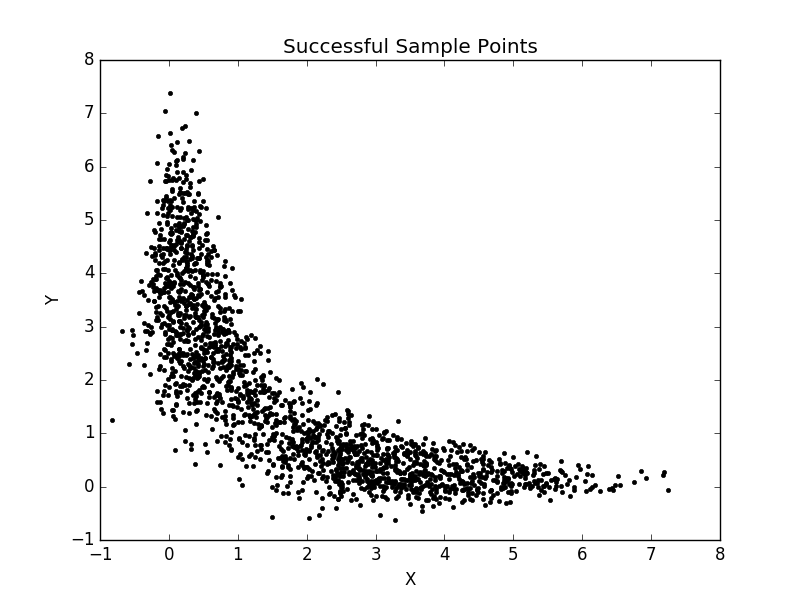
\includegraphics[scale=.5]{Pxy.png}
\caption{Probability Distribution Function $\pi(X,Y)$ with 2010 Successful Sample Points, and 10000 as Starting Number of points}
\end{figure}


\begin{figure}
\centering
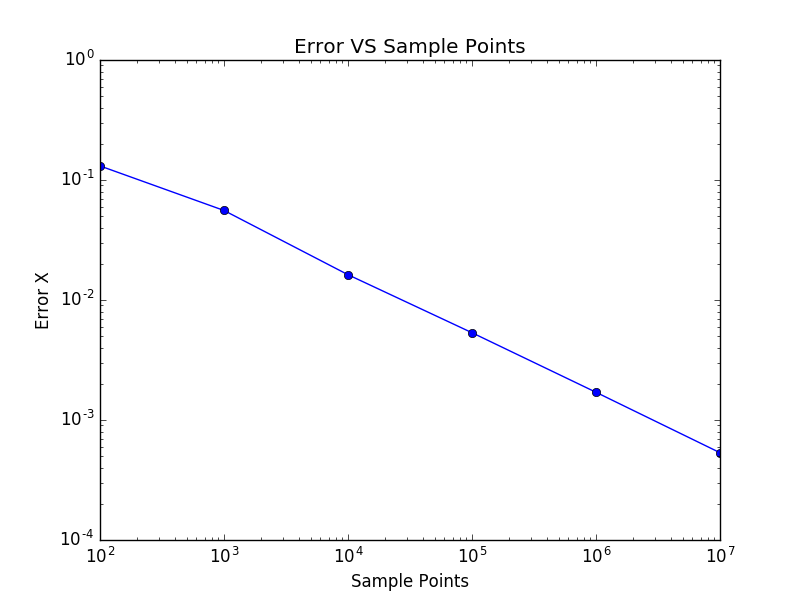
\includegraphics[scale=.5]{Error.png}
\caption{Accuracy of the MCMC Integral}
\end{figure}


\end{document}